\documentclass[article]{jss}
\usepackage{amsmath,amssymb,booktabs}

\author{Nicolas Salas\\INRAE}
\title{\pkg{remlax}: Automatic Differentiation for Restricted Maximum
       Likelihood, with a Structure Catalogue and a Choice of Engine}
\Plainauthor{Nicolas Salas}
\Plaintitle{remlax: Automatic Differentiation for REML}
\Abstract{
Fitting linear mixed models by restricted maximum likelihood is routine in
plant and animal breeding, but the software that covers the structures
breeders need---separable spatial fields, unstructured multi-trait
covariances, reduced-rank factor analytic models---is either proprietary or
requires the user to derive and code a likelihood by hand. \pkg{remlax} is a
free implementation that forms the marginal covariance explicitly and
differentiates it automatically, so that any structure added to its catalogue
receives its gradient for free. The same model specification is fitted by
either of two engines: a dense engine that differentiates $V$ and runs
unchanged on CPU or GPU, and a sparse engine built on the mixed model
equations for the subset of structures whose inverse is sparse and known in
closed form. Which engine is faster is not a matter of problem size: we show
that it is decided by where the density sits, and we give a structural
criterion that can be evaluated before any numerical work.
}
\Keywords{REML, mixed models, automatic differentiation, \proglang{JAX},
          variance components, spatial models, \proglang{R}, \proglang{Python}}
\Plainkeywords{REML, mixed models, automatic differentiation, JAX,
               variance components, spatial models, R, Python}
\Address{Nicolas Salas\\ E-mail: \email{nicolas.salas@supagro.fr}}

\begin{document}
\maketitle

\section{Introduction}\label{sec:intro}

% TODO(intro) — a rédiger en dernier, une fois les mesures complètes, pour que
% les promesses de l'introduction soient exactement celles que les sections
% suivantes tiennent.

\section{Model and parameterisation}\label{sec:model}

We consider the linear mixed model
%
\begin{equation}\label{eq:lmm}
  y = X\beta + \sum_{k=1}^{K} Z_k u_k + e,
  \qquad u_k \sim \mathcal{N}(0, G_k), \qquad e \sim \mathcal{N}(0, R),
\end{equation}
%
with marginal covariance $V = \sum_k Z_k G_k Z_k' + R$. The restricted
log-likelihood, up to an additive constant,
%
\begin{equation}\label{eq:reml}
  -2\log L_R(\theta) = \log|V| + \log|X'V^{-1}X| + y'Py,
  \qquad
  P = V^{-1} - V^{-1}X(X'V^{-1}X)^{-1}X'V^{-1},
\end{equation}
%
is a function of the variance parameters $\theta$ alone.

\subsection{One hand-written derivative rule}

The design decision from which everything else follows is that
\pkg{remlax} does not differentiate through the Cholesky factorisation of
$V$. It supplies the derivative of \eqref{eq:reml} with respect to $V$ in
closed form,
%
\begin{equation}\label{eq:vjp}
  \frac{\partial\,(-2\log L_R)}{\partial V} = P - (Py)(Py)',
\end{equation}
%
and lets automatic differentiation propagate that single rule backwards
through whatever code built $V$ from $\theta$.

Two consequences matter. Memory: reverse-mode differentiation through a
Cholesky factorisation stores the intermediates of the factorisation, whereas
\eqref{eq:vjp} needs $P$ and $Py$ only, so three $n \times n$ matrices are
live at once rather than a dozen. Genericity: a new covariance structure is a
new way of building $V$, and it receives its gradient without any further
derivation. The catalogue of Section~\ref{sec:catalogue} is a direct
consequence---adding a structure is writing its forward construction.

\section{The structure catalogue}\label{sec:catalogue}

A term contributes $Z_k (\Sigma_k \otimes C_k) Z_k'$ to $V$, where $\Sigma_k$
is a covariance between traits and $C_k$ a correlation between levels.
\pkg{remlax} parameterises the two independently: nine forms for $\Sigma$ and
twenty-five for $C$, so their product covers the models used in multi-trait
and spatial analyses without a combinatorial special case for each pairing.

\begin{table}[t]\centering
\begin{tabular}{llr}
\toprule
Form & Meaning & Parameters \\
\midrule
\code{iid}   & scalar variance                        & $1$ \\
\code{diag}  & heterogeneous variances, no correlation& $t$ \\
\code{us}    & unstructured                           & $t(t+1)/2$ \\
\code{fa}    & factor analytic, $m$ factors           & $tm + t$ \\
\code{rr}    & reduced rank, $m$ factors              & $tm$ \\
\code{chol}  & Cholesky parameterisation              & $t(t+1)/2$ \\
\code{ante}  & antedependence                         & $2t-1$ \\
\code{corh}  & common correlation, heterogeneous variances & $t+1$ \\
\code{fixed} & supplied, not estimated                & $0$ \\
\bottomrule
\end{tabular}
\caption{\label{tab:sigma}Covariance forms available for $\Sigma$.}
\end{table}

The level structures $C$ cover autoregressive and moving-average families
(\code{ar1}, \code{ar2}, \code{ar3}, \code{sar}, \code{ma1}, \code{ma2},
\code{arma}), isotropic and anisotropic metric kernels (\code{exp},
\code{gau}, \code{iexp}, \code{igau}, \code{ieuc}, \code{sph}, \code{cir},
\code{aexp}, \code{agau}, \code{mtrn}), correlation forms (\code{cor},
\code{corb}, \code{corg}), the separable product \code{ar1ar1}, and the
degenerate cases \code{id}, \code{fixed} and \code{own}.

\subsection{Reported scales}

% NOTE(mesure) — cette sous-section documente le comportement CORRIGÉ ce jour :
% les rapports rendent la valeur remise à l'échelle présente dans C, non la
% valeur transformée. Voir docs/structures.md, qui donne l'échelle rapportée
% famille par famille.

Every family is estimated on an unconstrained scale and reported on its
natural one. This matters for interpretation: a correlation is reported as the
rescaled value actually present in $C$, not as the transformed parameter the
optimiser moves. For the intrinsic metric kernels the sign of the range
parameter is not identified---$\theta$ and $-\theta$ give the same $C$---and
the reported value is taken positive.

\section{Two engines for one specification}\label{sec:engines}

\subsection{The dense engine}

The dense engine forms $V$ explicitly, factorises it, and applies
\eqref{eq:vjp}. It is written in \proglang{JAX} in double precision and runs
unchanged on CPU or GPU. Its cost is $O(n^3)$ per evaluation and it is
indifferent to how sparse the model is.

\subsection{The sparse engine}

The sparse engine never forms $V$. It works on the mixed model equations,
%
\begin{equation}\label{eq:mme}
  C = \begin{pmatrix} X'R^{-1}X & X'R^{-1}Z \\
                      Z'R^{-1}X & Z'R^{-1}Z + G^{-1} \end{pmatrix},
\end{equation}
%
which contain $G^{-1}$ and $R^{-1}$ rather than $G$ and $R$. It is built on
\pkg{RTMB} \citep{rtmb}, declaring both $\beta$ and $u$ as random so that the
Laplace approximation---exact for a linear Gaussian model---supplies the
sparse factorisation, the log-determinant and the exact gradient.

Its scope is a declared, testable rule rather than a heuristic: a model is in
scope when every level structure has a sparse inverse known in closed form.
Three qualify (\code{id}, \code{ar1}, \code{ar1ar1}), together with a
precision supplied directly by the user, and three covariance forms
(\code{iid}, \code{diag}, \code{us}). Everything else stays on the dense
engine. A consequence of the rule is that the sparse engine never inverts
anything: the retained structures have analytic inverses and analytic
log-determinants.

\subsection{Declaring a term by its precision}

A term may be declared by $K$, its between-level covariance, or by $K^{-1}$,
its precision. The second is the sparse route for a pedigree: Henderson's
rules give $A^{-1}$ directly, with about five non-zeros per individual,
without ever forming $A$ or factorising it. Supplying $K$ does not permit
this, since its Cholesky factor is dense and the inverse of a sparse matrix is
generally full. Supplying both is refused, and a precision that is itself
heavily filled---the genomic case---raises a warning, since sparsity buys
nothing there.

\section{Validation}\label{sec:validation}

% Chaque affirmation de cette section renvoie au fichier qui la produit.
% Aucune n'est reprise d'une exécution antérieure non versionnée.

Validation is organised around what a failure would have meant, not around
test counts. Three levels are used, and the third is the one that found
defects the other two could not.

\subsection{Internal agreement}

\emph{tests/R/test\_remlax\_tmb\_parity.R} checks that the two engines read
$\theta$ identically: that $\Sigma(\theta)$ agrees for \code{iid},
\code{diag} and \code{us}; that the closed-form \code{ar1} and \code{ar1ar1}
precisions are exact inverses of the correlation matrices the dense engine
builds, verified by forming $K^{-1}K$ rather than by inspecting a sparsity
pattern; and that the analytic log-determinants agree with numerical ones.
Thirty checks, largest discrepancy $3.6 \times 10^{-15}$.

\subsection{Cross-engine agreement, in both directions}

\emph{tests/R/test\_remlax\_tmb\_vs\_dense.R} evaluates each engine at the
other's optimum. Both directions are needed: an engine could have a correct
surface along the other's path and be wrong elsewhere. Sixteen checks over
four designs agree to $10^{-12}$ on cross-evaluation and $6 \times 10^{-9}$ on
the attained optima.

\subsection{An arbiter beholden to neither engine}

Two engines that agree prove less than one engine checked against an
independent computation. \emph{tests/R/test\_remlax\_tmb\_prec.R} carries a
REML likelihood written out in dense linear algebra, and it settled three
disagreements during development that engine-to-engine comparison could not.
In one of them it identified the sparse engine as wrong; in another, the dense
engine; in the third, the test design itself.

The defect it caught in the precision path deserves reporting, because it is
the class of defect an estimate-based test cannot see. The objective read a
user-supplied log-determinant field and silently fell back to zero when
absent, so $\log|K|$ was simply missing. Being constant, the omission left the
gradient untouched: the parameter estimates agreed to five digits and only the
likelihood was wrong---hence every model comparison, likelihood ratio test and
information criterion computed from it.

\subsection{Agreement with established software}

Against \pkg{asreml} 4.2 \citep{asreml}, \pkg{lme4} \citep{lme4} and
\pkg{sommer} \citep{sommer}, in a container where all are installed:
restricted log-likelihoods agree to $10^{-5}$ in \pkg{asreml}'s own
convention, variance components to the same order, and heritabilities with
their delta-method standard errors.

BLUPs are checked separately, in
\emph{tests/R/test\_remlax\_asreml\_blup.R}, because they are the output a
breeder actually uses and no earlier suite touched them. Matching levels by
name rather than by position, all $60$ predictions agree with \pkg{asreml} to
$3.2 \times 10^{-6}$, with a correlation of $1$ to twelve digits, and the
fixed effect to ten.

That test also records a gap rather than a disagreement: \pkg{remlax} computes
BLUPs but does not expose their prediction error variances, where
\pkg{asreml} reports a standard error and a $z$ ratio for every effect.
Without them a candidate ranking carries no measure of reliability, so this is
a required addition, and the information is available since the solver already
factorises the coefficient matrix.

\subsection{A conditioning limit, made deliberate}

The mixed model equations \eqref{eq:mme} contain $R^{-1}$, so the sparse
engine degrades as the residual variance approaches zero. Rather than hope an
optimiser visits that region, the check imposes $\theta$ and reports the
degradation, which is monotone: at $\sigma_e^2 = 3.4 \times 10^{-4}$ the two
engines agree to $3.8 \times 10^{-11}$, and at $3.8 \times 10^{-11}$ they
agree only to $1.7 \times 10^{-4}$. This is structural to the formulation,
and it is why \pkg{asreml} parameterises the ratio of variances instead.

\section{Performance}\label{sec:performance}

\subsection{Measurement protocol}\label{sec:protocol}

Four points of protocol are stated here because each of them changed a
conclusion during development.

First, and most consequentially: \emph{fit times are not compared across
backends}. The two backends follow different optimisation trajectories on the
same model---419 iterations on the card against 317 on the CPU, reaching the
same optimum to $8.6 \times 10^{-10}$ relative. Floating-point addition is not
associative, so a reduction ordered across thousands of GPU threads differs in
its last bits from one ordered across sixteen CPU cores; the line search then
accepts a different step, and the paths diverge. Near a flat optimum the
stopping test operates at that noise floor. A total time therefore mixes a
hardware cost with a path length settled by rounding noise, and the mixture is
not separable after the fact.

The paired unit is instead an \emph{objective evaluation at an imposed}
$\theta$, which performs identical arithmetic on both devices. The imposed
$\theta$ need not be the optimum: the cost of a Cholesky factorisation depends
on dimensions, not values, so any $\theta$ common to both sides makes the
comparison valid, and none has to be bought with a reference fit.

Every GPU figure reported below is measured on a \emph{whole} A100. Earlier
sweeps used a one-seventh MIG slice, and we had assumed the slice figures
could be treated as a fixed pessimistic bound. They cannot: measured on the
same script, the slice-to-card ratio is not constant.

\begin{table}[h]\centering
\begin{tabular}{rrrr}
\toprule
$n$ & Slice (s) & Whole card (s) & Ratio \\
\midrule
\phantom{0}\phantom{0}250 & \phantom{00}0.32 & \phantom{0}0.28 & 1.16 \\
\phantom{0}1000 & \phantom{00}0.40 & \phantom{0}0.32 & 1.23 \\
\phantom{0}2000 & \phantom{00}1.26 & \phantom{0}0.65 & 1.94 \\
\phantom{0}4000 & \phantom{00}6.39 & \phantom{0}1.73 & 3.69 \\
\phantom{0}8000 & \phantom{0}94.19 & 15.49 & 6.08 \\
12000 & 294.75 & 41.88 & 7.04 \\
\bottomrule
\end{tabular}
\caption{\label{tab:slice}A one-seventh slice against the whole card, same
script. The ratio rises from $1.16$ to $7.04$ and never approaches the
compute-unit ratio of $15.4$: below $n \approx 2000$ the fixed costs dominate
and a bigger card buys almost nothing, while above $n = 8000$ the
factorisation is bandwidth-bound rather than unit-bound.}
\end{table}

One practical consequence is worth stating for users of shared hardware: for
several independent models of moderate size, seven slices beat one whole
card, and the reverse holds beyond $n = 8000$.

Second, each grid cell is measured in a \emph{fresh process}. A sweep that
measures all cells in one process reuses compiled programs across cells, so
execution order influences the result---in an earlier sweep the compilation
column fell from $79$\,s to $2.7$\,s on the late cells for that reason.

Third, cell names below are written out rather than abbreviated: a
\emph{case} is the structure of the data (a separable \code{ar1} field, or a
full genomic kinship), and an \emph{engine} is what fits it. The two are
crossed, so a structurally dense case can be forced onto the sparse engine---a
cell its declared scope excludes, measured here to price the wrong choice
rather than assert it.

\subsection{Where the two devices differ}\label{sec:paired}

Six model families were measured, chosen because they are what plant breeders
actually fit rather than because they are convenient to generate: single-trait
genomic prediction; multi-trait and multi-environment covariances under
\code{iid}, \code{diag}, reduced-rank \code{fa} and unstructured \code{us} at
two, four and six traits; a row-by-column field trial with a separable
\code{ar1} residual; and a direct-and-indirect effects design whose indirect
incidence is column-dense. Each family was crossed with an identity
relationship matrix and with a dense genomic one---the structural axis---at
$n$ from $2000$ to $16\,000$, five repetitions per cell.

Figure~\ref{fig:backend} reports the result. The dense engine is
\emph{indifferent to the structure of the model}: at $n = 8000$, across every
family, every covariance structure and both relationship matrices, an
evaluation costs between $0.219$ and $0.282$\,s---a factor $1.3$ between the
extremes, against a factor of four in the parameter count and two regimes of
kinship. This is the central asymmetry of the paper stated as a measurement
rather than an argument. The engine forms and factorises $V$ whatever the
sparsity of the model, which is precisely why it wins when the model is dense
and loses when it is sparse.

Evaluation cost is sub-cubic and becomes less so with size: the median rises
by $3.8$, then $5.2$, then $6.0$ per doubling of $n$, against $8$ for a pure
Cholesky. Below $n \approx 4000$ the card is not saturated and fixed launch
costs dominate; by $n = 16\,000$ it approaches its compute limit.

The median speed-up of the whole card over sixteen CPU cores, on $87$ paired
cells, is $27.2$, $26.8$, $29.7$ and $21.7$ at $n = 2000$, $4000$, $8000$ and
$16\,000$. It is therefore flat across the range \emph{of this design}: the card does not
win by more as the problem grows, the two curves being close to parallel.

That qualification is not a formality, and a second design contradicts the
unqualified reading. Section~\ref{sec:traits} grows the problem by adding
traits at a fixed number of observations per trait and a fixed number of
levels, and there the speed-up rises steeply---$21$, $42$, $64$ at
$n = 2000$, $4000$, $6000$. At $n = 4000$, common to both designs, one gives
$27$ and the other $42$. The difference is what happens to the effect vector:
the sweep here scales the number of levels with $n$, whereas the trait sweep
holds it fixed, so the two designs load the two devices differently at equal
$n$. The speed-up is thus a property of the design, not a constant of the
hardware, and quoting a single number for it---as software papers routinely
do---is the mistake this pair of sweeps was built to expose. Kinship does not move it either: on the multi-trait family, the only one
sampled densely enough to support the comparison, the median is $26.9$ without
a genomic relationship matrix and $28.2$ with it, on $28$ paired cells each.

Two limitations are stated rather than left to inference. The CPU cells at
$n = 8000$ and $16\,000$ were recovered from the run logs of two jobs that
exhausted their walltime before writing their result files---a single fit at
$n = 16\,000$ with six traits took $2736$\,s---so those two sizes carry $12$
and $11$ cells against $32$ at the smaller sizes, and no full fits. And the
CPU points scatter over a factor of $13$ at $n = 2000$ where the card holds
within $1.3$; that dispersion is contention on a shared node rather than a
property of the model. It shrinks to a factor of $1.3$ at $n = 16\,000$, where
computation dominates and the node's other tenants matter less---which is the
evidence that it is noise and not signal.

\begin{figure}[t]\centering
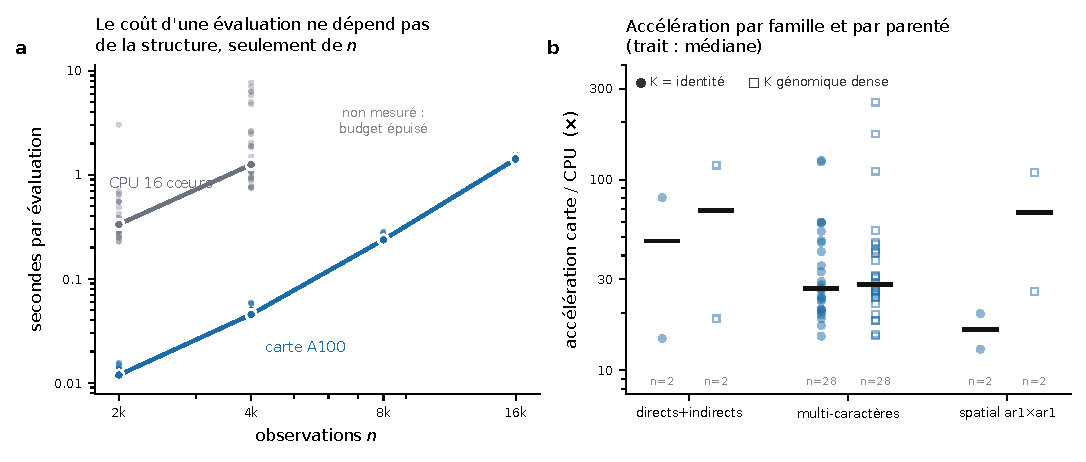
\includegraphics[width=\textwidth]{figures/fig_backend.pdf}
\caption{\label{fig:backend}Paired evaluation cost at an imposed $\theta$.
\textbf{(a)} Each point is one cell---one family, one covariance structure,
one relationship matrix; the line joins the medians. The card's cells collapse
onto each other at every size, so the engine's cost is set by $n$ alone.
\textbf{(b)} Card-over-CPU speed-up, one point per paired cell, with the
number of pairs printed at each size; the bar is the median. The medians are
$27.2$, $26.8$, $29.7$ and $21.7$: the advantage is a constant factor, not one
that widens with the problem. The two largest sizes carry fewer pairs because
their CPU measurements were recovered from the logs of jobs that exhausted
their walltime.}
\end{figure}

\subsection{Adding traits: the design a breeder runs}\label{sec:traits}

The two sweeps above hold the total number of observations fixed and vary the
covariance structure within it. That isolates the axes but it is not what
happens in a breeding programme, where traits are added to a trial that
already exists: the same plants, measured for more things. The third sweep
follows that shape---an unstructured $\Sigma$ over $t$ traits, $2000$
observations per trait, $500$ levels, $t$ from $1$ to $8$---so $p = t(t+1)/2$
rises from $1$ to $36$ while $n$ rises with it. The axes are deliberately
coupled here; it is the pair of designs that separates them.

Three cells exist, not four. The sparse engine factorises through
\pkg{CHOLMOD}, which is CPU-only, so \emph{sparse} and \emph{GPU} are mutually
exclusive and the engine choice is a trade-off rather than two independent
options. That empty cell is a result, and it is stated rather than left as a
gap in a table.

Two findings so far, on the completed whole-card lot and a partial read of the
CPU lots still running.

\emph{The two devices are on different slopes.} Over $n = 2000$ to $6000$ an
evaluation costs $n^{2.78}$ on sixteen CPU cores against $n^{1.77}$ on the
card; over the card's full range to $n = 16\,000$ the exponent rises to
$2.14$. The card is not saturated at the small sizes---fixed launch costs it
does not amortise until later---while the CPU is already compute-bound. The
speed-up therefore grows roughly linearly in $n$ over this range, which is the
disagreement discussed in Section~\ref{sec:paired}.

\emph{Iterations stop growing.} The card lot gives $6$, $15$, $24$, $36$, then
$32$, $32$, $37$, $33$: from $t = 4$ to $t = 8$ the parameter count is
multiplied by $3.6$ and the iteration count does not move. The pooled slope of
$p^{0.47}$ across the whole sweep is carried entirely by the rise up to
$t = 4$. Read against the fixed-$n$ sweep, where iterations \emph{did} grow
with $p$, this suggests that the extra data arriving with each trait sharpens
the optimum enough to offset the extra dimension. Two designs are consistent
with that reading; neither establishes it, and we record it as a hypothesis.

A third result arrives as a by-product and is worth more than either, because
it re-tests the paper's central claim on a design built for something else:
a dense genomic relationship matrix changes the cost of an evaluation by at
most $2.2\%$ across seven matched pairs on both devices. The dense engine's
indifference to model structure was measured in Section~\ref{sec:paired} and
is reproduced here without having been aimed at.

\begin{figure}[t]\centering
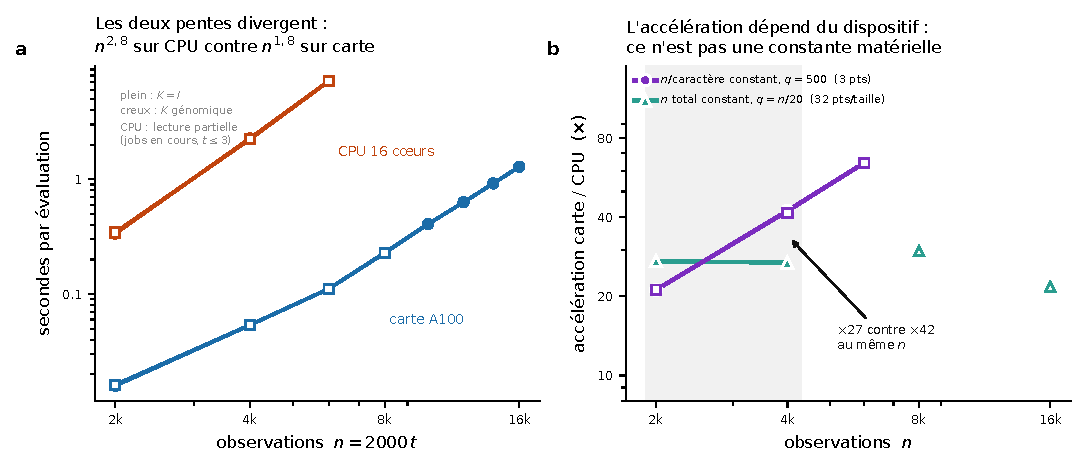
\includegraphics[width=\textwidth]{figures/fig_traits.pdf}
\caption{\label{fig:traits}Adding traits at constant observations per trait.
\textbf{(a)} Cost of one evaluation at an imposed common $\theta$; filled
markers are an identity relationship matrix, open markers a dense genomic one,
and the two coincide. The CPU series is a partial read of jobs still running
and stops at $t = 3$. \textbf{(b)} The card-over-CPU speed-up from this design
against the same quantity from the fixed-$n$ design of
Section~\ref{sec:paired}. They disagree in the shaded region where both were
measured, which is why no single speed-up figure is quoted anywhere in this
paper.}
\end{figure}

\subsection{The parameter count is not a measure of difficulty}\label{sec:paxis}

The number of covariance parameters $p$ ranged from $3$ to $27$ across the
sweep, varied through the number of traits and through the covariance
structure. Its two effects separate cleanly, and only one of them is the one
usually assumed.

On the cost of a single evaluation, $p$ has \emph{no} effect. Fitting a power
law to the $28$ cells at $n = 8000$ gives an exponent of $0.000$: at $p = 3$
an evaluation costs $0.2384$\,s and at $p = 27$ it costs $0.2316$\,s. This is
expected---the factorisation of $V$ does not know how many parameters
generated it---but it is worth measuring, because it means the parameter count
enters the total only through the number of evaluations.

On that number, the naive reading is wrong, and pooling the structures
produces it. Regressed over every multi-trait cell, iterations scale as
$p^{0.95}$, near-linear and tidy. Split by structure family the exponent is
$0.01$ for \code{iid}, $0.27$ for \code{diag}, $0.44$ for \code{us} and
$1.01$ for \code{fa}: the pooled slope was an artefact of the reduced-rank
cells occupying the high-$p$ end. The clearest statement of this is a direct
comparison at six traits, where \code{fa(6,2)} carries $23$ parameters and
needs $154$ iterations while \code{us(6)} carries $27$ and needs $34$. More
parameters, four and a half times fewer iterations.

The consequence for the decision rule in Section~\ref{sec:decision} is that
$p$ cannot be used as a scalar measure of how hard a model is to fit. A
reduced-rank structure buys parameter economy and pays for it in path length,
and any predictor that reads only the count will misprice it by a factor of
several. The structure family must enter the rule alongside the count.

\begin{figure}[t]\centering
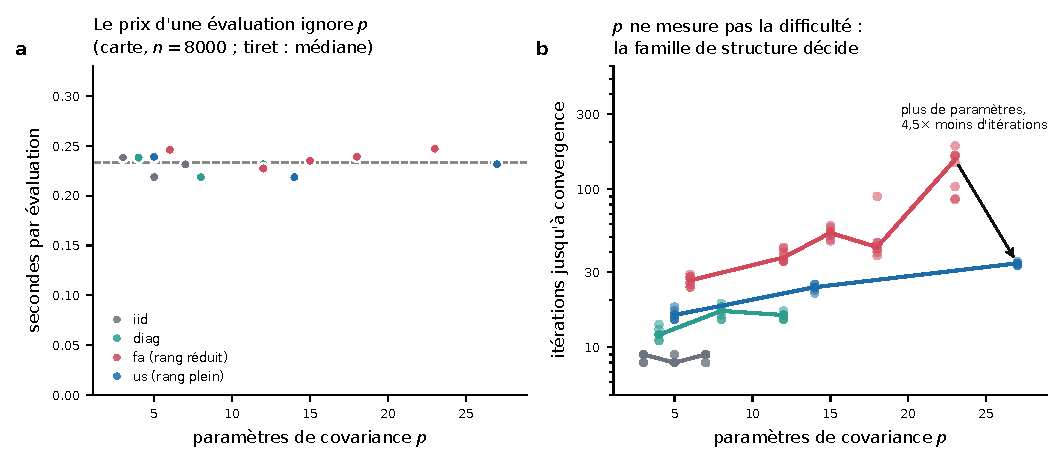
\includegraphics[width=\textwidth]{figures/fig_axe_p.pdf}
\caption{\label{fig:axep}The two effects of the parameter count, measured on
the whole card. \textbf{(a)} At fixed $n$, an evaluation costs the same
whatever $p$ and whatever the structure; the dashed line is the median over
all $28$ cells. \textbf{(b)} Iterations to convergence against $p$, one point
per fit and a line through the medians, coloured by structure family. The
families diverge, and the arrow marks the pair that refutes reading $p$ as
difficulty.}
\end{figure}

\subsection{Which engine, and on which device}\label{sec:decision}

The trait sweep measures all three cells that exist, and the answer is not the
one an accelerator invites. Across $t = 1$ to $8$ the sparse engine on sixteen
CPU cores is faster than the dense engine on a whole A100 at every size, and
the margin widens: $22\times$ to $121\times$ per evaluation at the imposed
common $\theta$, and $7\times$ to $78\times$ for a complete fit
(Figure~\ref{fig:moteurs}). There is no crossover to report.

The three exponents say why. Over this range an evaluation costs $n^{2.78}$ for
the dense engine on CPU, $n^{2.14}$ for the same engine on the card, and
$n^{1.25}$ for the sparse engine. The gap is algorithmic, not hardware: the
sparse factorisation pays only for the fill it actually incurs, while the dense
engine forms and factorises the whole of $V$ regardless of sparsity. The
indifference to model structure established in Section~\ref{sec:paired} is an
advantage on dense models and precisely this liability on sparse ones.

The empty fourth cell then decides the practical recommendation. Since
\pkg{CHOLMOD} runs on the CPU, \emph{sparse} and \emph{GPU} cannot be combined:
for any model inside the sparse engine's declared scope the right choice is the
CPU, and the accelerator earns its place only on models the scope excludes ---
metric kernels, factor-analytic structures, a supplied dense relationship
factor. That is a narrower role for the GPU than we expected when this work
started, and it is the honest reading of the measurements.

Two components of the comparison were wrong until they were checked, both in
the direction that flattered the dense engine, and both are recorded because
the corrected figures depend on them. The sparse engine computed \pkg{TMB}'s
standard-error report on every fit --- the covariance of all random effects,
which the dense call never forms --- costing $42\%$ of the sparse fit time at
$t = 8$; and its iteration cap was $300$ against the dense engine's $3000$,
which would have let a truncation read as a convergence. Both are corrected in
the figures above.

What the cost model still does not explain, we name rather than absorb into a
fitted constant: construction plus counted evaluations account for only $15$ to
$48\%$ of a sparse fit. The remainder is the gradient evaluations, which
\pkg{nlminb} requests about as often as the objective, and instrumenting them
is the next step rather than a closed question.

\begin{figure}[t]\centering
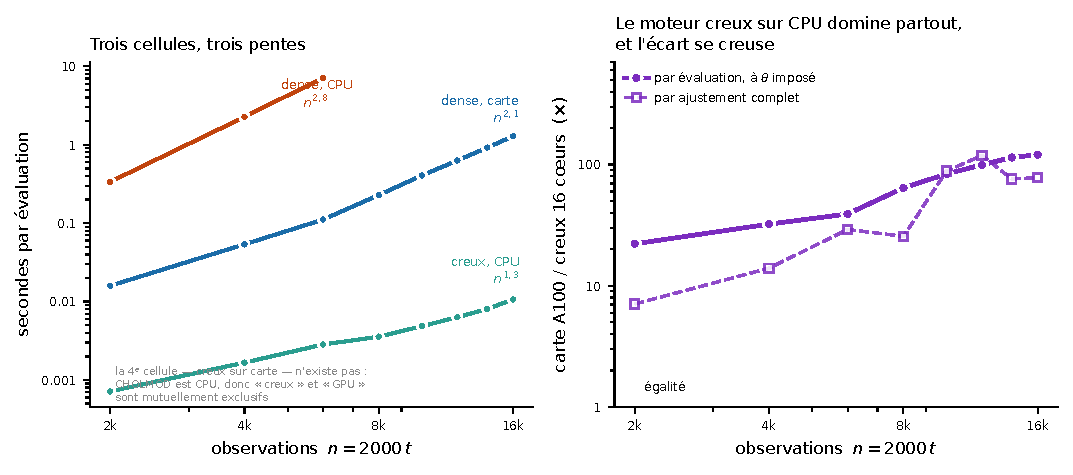
\includegraphics[width=\textwidth]{figures/fig_moteurs.pdf}
\caption{\label{fig:moteurs}The three cells that exist.
\textbf{(a)} Cost of one evaluation against problem size, with the fitted
exponent for each cell; the fourth cell---sparse on the card---does not exist,
\pkg{CHOLMOD} being CPU-only. \textbf{(b)} Whole-card dense engine over
sixteen-core sparse engine, per evaluation and per complete fit. The dotted
line is equality and is never approached. The fit ratio sits below the
evaluation ratio because most of a sparse fit is gradient evaluations rather
than objective evaluations.}
\end{figure}

\subsection{A cost model that can be, and was, refuted}\label{sec:reconstruction}

The measurements above decompose a fit into three parts: a compilation paid
once, the cost of one evaluation, and a number of evaluations. That
decomposition is only useful if the three reconstruct the total, so we tested
it, and it failed. Across the $32$ paired CPU cells at $n = 2000$ the ratio of
predicted to measured time was $0.48$ in median: the model accounted for half
the time.

The cause was not in the timing but in the count. We had \emph{predicted} the
number of evaluations as $n_{\text{iter}} + 2p$---the iterations plus the
finite-difference Hessian---whereas the bounded quasi-Newton optimiser performs
several evaluations per iteration inside its line search, and each Newton
polish step adds a full Hessian of its own. Measured on a case with $p = 14$
and $32$ iterations: $60$ predicted, $102$ actual. The solver now counts its
own calls to the objective. With the true count the reconstruction reaches
$0.94$; the residual six per cent is incidence assembly, the starting value,
and the predictors.

We report the failure because the alternative was available and worse. A
multiplicative correction of $1.70$ would have closed the budget exactly while
concealing the missing term, and a cost model calibrated that way predicts
correctly on the grid it was fitted to and nowhere else.

\subsection{An external contrast that does not replicate}\label{sec:external}

\pkg{ASReml} partitions the terms of a model into a dense set, whose
coefficient-matrix inverse is fully formed, and a sparse set, for which it is
formed only partially; a random term may be moved into the dense set
explicitly, and the manual recommends this for relationship matrices of the
order of several thousand. This offers a contrast internal to one program:
same model, same data, same optimiser, only the solve path differing.

It does not reproduce the asymmetry we report. On a dense genomic relationship
matrix at $n = 8000$, with three repetitions, the sparse-to-dense time ratio
was $0.97$, $1.01$, $1.04$ and $1.02$ at $q = 500$, $1000$, $2000$ and $4000$:
no measurable advantage either way. Log-likelihoods and iteration counts were
identical between the two paths throughout, so the partition changes the
solution route and not the problem---but on this model it changes the cost by
less than the measurement noise.

One caveat we cannot close: ``the partition has no effect'' and ``the option
did not apply'' would look alike here. The evidence that it applied is thin
but real---the median prediction error variances agree bit-for-bit at
$q = 500$ and $1000$ and differ in the tenth digit at $q = 2000$ and $4000$,
the signature of a different arithmetic path rather than of no path at all.

This measurement also retires an explanation we had found attractive. Because
the inverse is only partially formed for sparse terms, we expected prediction
error variances to be unavailable on the sparse side, and to be able to
present \pkg{remlax}'s lack of them as the same structural price. They come
back from both paths, with median standard errors agreeing to ten digits.
\pkg{remlax} not exposing prediction error variances is an implementation gap,
and is recorded as one.

\subsection{Fixed costs, and an unfavourable comparison}\label{sec:fixed}

A reader comparing \pkg{remlax} to established software on a small model will
find it slower, and by a wide margin. We report that measurement first,
because the decomposition behind it is the informative part.

On a single-trait model with $720$ observations, $60$ genotypes and two
variance parameters, \pkg{asreml} fits in $0.080$\,s. \pkg{remlax} takes
$3.40$\,s called from \proglang{R}. Decomposing that figure:

\begin{table}[h]\centering
\begin{tabular}{lrr}
\toprule
Quantity measured & Time & Ratio to \pkg{asreml} \\
\midrule
Wall time, called from \proglang{R}          & 3.398\,s & 42.5 \\
Fit in process                               & 1.329\,s & 16.6 \\
Internal time reported by the solver         & 0.598\,s & \phantom{0}7.5 \\
Algebraic cost alone ($9 \times 0.0137$\,s)  & 0.123\,s & \phantom{0}1.5 \\
\bottomrule
\end{tabular}
\caption{\label{tab:fixed}Where the time goes on a small model. The linear
algebra is within a factor of $1.5$; everything above it is fixed cost.}
\end{table}

Compilation, the finite-difference Hessian and the BLUPs account for
$90.7\,\%$ of the in-process fit, and the \proglang{R} interface adds $2.8$\,s
of out-of-process invocation because it launches a \proglang{Python} process
per fit. On a model with two parameters and nine iterations there is nothing
to amortise these costs against.

This unifies the section. Fixed costs are amortised over evaluations, and the
number of evaluations is governed by the number of parameters, so
\pkg{remlax} becomes competitive exactly when a model is large enough in
parameters to pay for its own setup---the same criterion as for compilation in
Section~\ref{sec:performance}. It also identifies the most valuable
optimisation in the package, which is not algebraic: a persistent worker
process reused across fits would remove the $2.8$\,s entirely, and it matters
most for the serial-fitting workloads (likelihood ratio tests over many
reduced models) where hundreds of fits are performed.

\subsection{Compilation is a purchasable cost, not a fixed one}

\pkg{remlax} compiles the model to a program before evaluating it, and that
compilation runs on the CPU whichever device the program targets. On a
dense-kinship model with $n = 2000$ and $q = 1000$:

\begin{table}[h]\centering
\begin{tabular}{rrrr}
\toprule
Cores & CPU backend & GPU backend & Backend gap \\
\midrule
 2 & \phantom{0}75.99\,s & \phantom{0}79.89\,s & 5.1\,\% \\
 8 & \phantom{0}20.95\,s & \phantom{0}21.49\,s & 2.6\,\% \\
16 & \phantom{0}10.88\,s & \phantom{0}12.24\,s & 12.6\,\% \\
\bottomrule
\end{tabular}
\caption{\label{tab:compil}Compilation time against core count. Eight times
the cores divide the cost by 7.0---87\,\% parallel efficiency---while the
target device changes it by at most 13\,\%.}
\end{table}

Two practical consequences follow, and the second is counter-intuitive.
Compilation is amortised over evaluations, so it is negligible for a model
with many parameters and dominant for a model with few: the break-even is
counted in evaluations, not in problem size. And a GPU job should request many
CPU cores; fitting several models concurrently on separate GPU slices with few
cores each is slower than fitting them sequentially with all cores.

\subsection{Where each engine wins}

% TODO(mesure) — tableau à compléter par le criblage G x R et par la carte
% entière. Les cellules ci-dessous sont mesurées et versionnées dans
% benchmarks/results/.

For a structurally sparse model the sparse engine wins by a wide margin: at
$n = 4000$ it fits in 2.6\,s against 608\,s for the dense engine on CPU, a
factor of 230. For dense genomic kinship the picture is not the one the
folklore suggests---the sparse engine still wins most cells, and loses only
when the number of effects is large relative to the number of observations.
What separates the two is that the sparse engine's cost is governed by $q$ and
is flat in $n$ (2.43, 2.43 and 2.39\,s per evaluation at $q = 500$ for
$n = 1000, 2000, 4000$), while the dense engine's cost grows with $n$.

\subsection{The empty cell}

The sparse engine has no GPU path, and this is not an omission. Sparse
factorisation goes through \pkg{CHOLMOD}, which is CPU-only, and the reason is
structural: irregular memory access and the sequential dependencies of the
elimination tree give it low arithmetic intensity, where a dense product
reaches close to peak. Sparse and GPU are therefore mutually exclusive rather
than two independent axes, which turns the choice of engine into an arbitrage.

\section{Choosing an engine}\label{sec:decision}

% TODO(mesure) — cette section attend le criblage G x R. La prédiction qu'elle
% teste est écrite ici AVANT la mesure, pour qu'elle soit réfutable.

The criterion is structural and costs no numerical work. What decides is not
the size of the problem but where the density sits. In \eqref{eq:mme}, a dense
$G$ fills its own block, from which fill propagates through elimination; a
dense $R$ fills $Z'R^{-1}Z$ for every term at once, including terms whose
precision is diagonal. The prediction, which the accompanying screening tests
at matched parameter counts, is that an unstructured residual disqualifies the
sparse route where a dense genomic kinship does not.

\section{Outlook}\label{sec:outlook}

Three directions are identified by measurement rather than by preference.

Relationship matrices currently enter the compiled program as constants---the
compiler reports 2.17\,GB captured on a real multivariate analysis---so the
program is recompiled for every size. Passing them as arguments would compile
once and reuse, and the gain is measurable against the figures of
Section~\ref{sec:performance}.

Prediction error variances for BLUPs are computed but not yet confronted with
a reference implementation.

Finally, the sparse route is limited by the CPU-only factorisation. A
matrix-free formulation---for Markov random field representations of spatial
fields in particular---would restore a GPU path, at the cost of a stochastic
gradient and hence of a different stopping rule.

\bibliography{remlax}

\end{document}
